\subsubsection{Optimization Objective}
\begin{itemize}[--]
	\item In logistic regression we had the sigmoid activation function, and the hypthosis: $h(x)=\frac{1}{1+e^{-\theta^T x}}$
	\item If we have an example where $y=1$, we want $h(x)=1$, this implies $\theta^{T}x \gg 0$
	\item Conversly, if $y=0$, we want $h(x)=0\to \theta^{T}x\ll 0$
	\item When $y=1$ only the first term of the cost function wil matter ($-y\log\frac{1}{1+e^{-\theta^T x}}$)
	\item If we plot this as a function of $z=\theta^T x$ we get the  following curve
	\begin{center}
		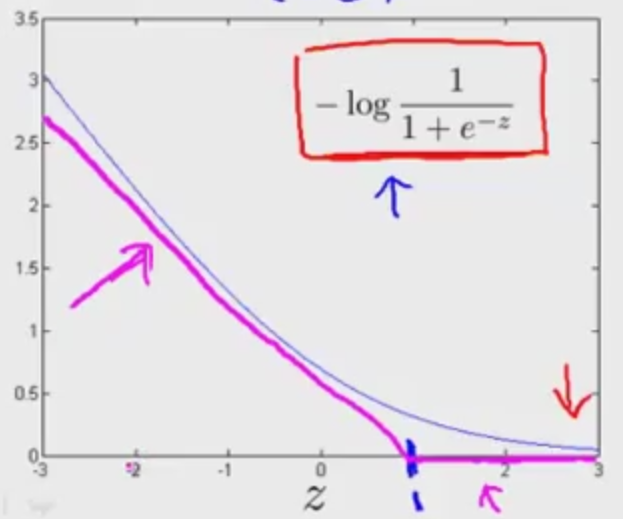
\includegraphics[scale=0.5]{sections/cs229/w9/y_1.png}
	\end{center}
	\item The purple line will be our SVM's cost when $y=1$, which is made up of two line segments

	\item Similarly for when $y=0$ (second term of cost function) we have the same following graphs:
	\begin{center}
		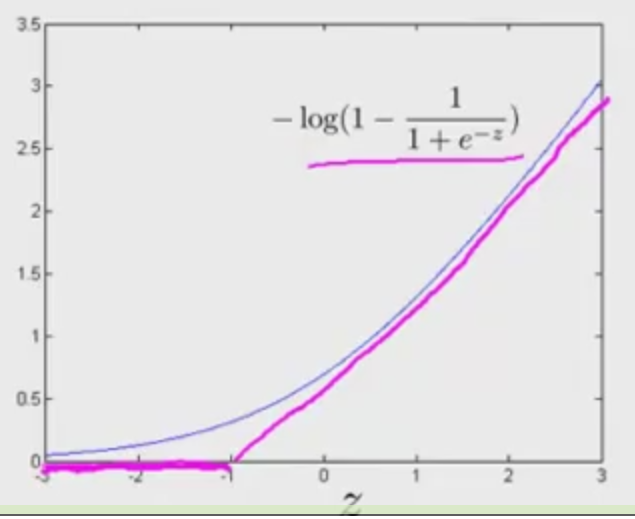
\includegraphics[scale=0.5]{sections/cs229/w9/y_2.png}
	\end{center}

	\item We will denote the SVM's cost when $y=0$ to be $\text{cost}_1 (z)$, similarly when $y=0$, $\text{cost}_0 (z)$
	\item Logistic regression's cost function:
		$$\min_{\theta}\frac{1}{m} \left[ \sum_{i=1}^{m} y^{(i)} (-\log{h(x^{(i)})}) + (1-y^{(i)})((-\log{1-h(x^{(i)})}))\right] + \frac{\lambda}{2m}\sum_{j=1}^{n}\theta_{j}^{2}$$
	\item Support vector machine's cost function:
		$$\min_{\theta}\frac{1}{m} \left[ \sum_{i=1}^{m} y^{(i)} \text{cost}_1(\theta^{T}x^{(i)}) + (1-y^{(i)})\text{cost}_0 (\theta^{T}x^{(i)})\right] + \frac{\lambda}{2m}\sum_{j=1}^{n}\theta_{j}^{2}$$
	\item We should be able to remove the constant, since the minimization problem will take care of reducing it:
		$$\min_{\theta} \left[ \sum_{i=1}^{m} y^{(i)} \text{cost}_1(\theta^{T}x^{(i)}) + (1-y^{(i)})\text{cost}_0 (\theta^{T}x^{(i)})\right] + \frac{\lambda}{2}\sum_{j=1}^{n}\theta_{j}^{2}$$
	\item Also, for SVM we will use a different parameter to control the weight of the penalty term: $A+\lambda B\to CA+B$, where $C$ is our new term
	\item Having learned the parameters $\theta$, this is the hypothesis for the SVM:
		$$
			h(x)=\begin{cases}
				1 & \text{if } \theta^{T}x\geq 0 \\
				0 & \text{otherwise}
			\end{cases}
		$$
\end{itemize}

\subsubsection{Large Margin Intuition}
\begin{itemize}[--]
	\item -
	\begin{center}
		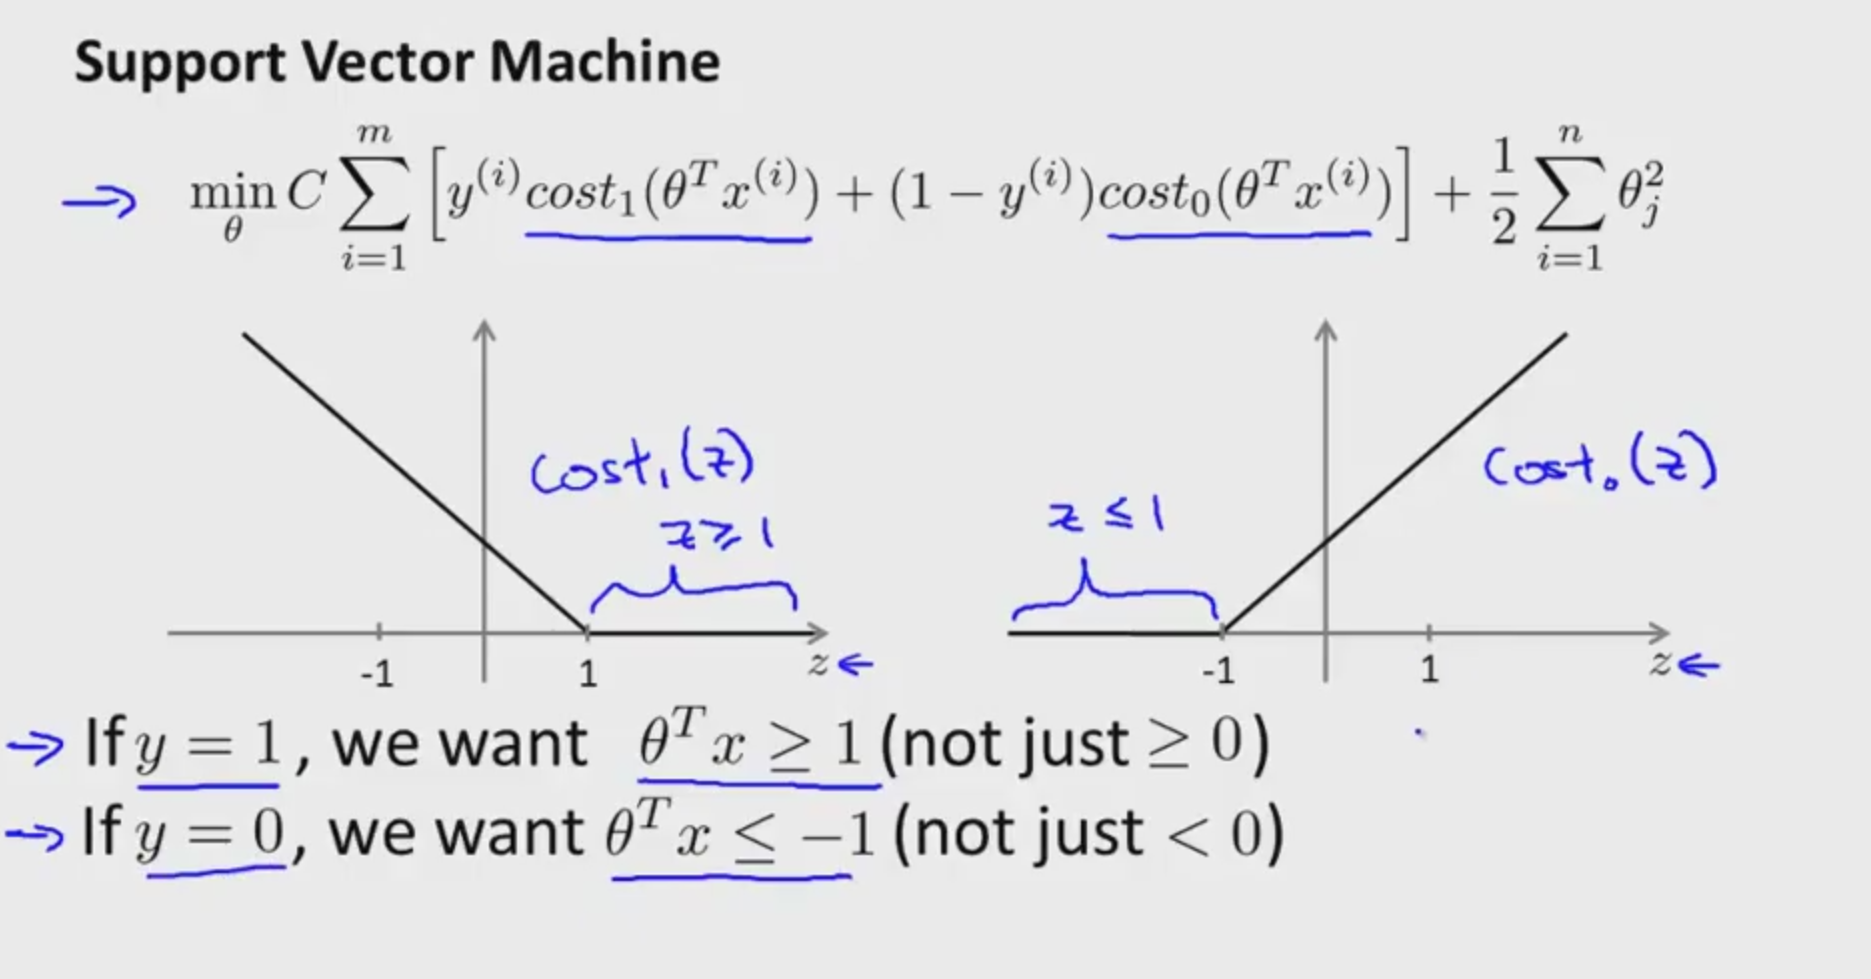
\includegraphics[scale=0.5]{sections/cs229/w9/svm.png}
	\end{center}

	\item To make these cost functions small, we want:
	\begin{align*}
		\theta^{T}x\geq 1 &\text{If } y=1 \\
		\theta^{T}x\leq -1 &\text{If} y=0
	\end{align*}

	\item However, if you just barely get the example right (0 instead of +/- 1), where you stlil have some cost
	\item This builds an extra safety margin factor, still predicting the correct result but there's another ``level'' where you will have no cost
	\item If $C$ is very large, and we want our first cost term to be 0, so our resulting cost function is:
		$$\min_{\theta}\frac{1}{2}\sum_{i=1}^{n}\theta_{j}^{2}$$
	\item This is subject to the constraint: 
	\begin{align*}
		\theta^{T}x^{(i)}\geq 1  & \text{if } y^{(i)}=1\\
		\theta^{T}x^{(i)}\leq -1 & \text{if } y^{(i)}=0
	\end{align*}

	\item When you solve this optimization problem, you get a linearly separable example sets (can be divided by lines into their classes).
	\begin{center}
		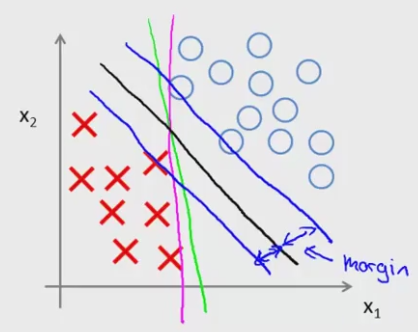
\includegraphics[scale=0.5]{sections/cs229/w9/margin.png}
	\end{center}

	\item There exists many different lines (green/purple) that can fit this division; however, the svm will find the black (most natural looking) dividing line
	\item This line has the largest margin from the classes (the blue lines)
	\item The distance from the predicted line and the nearest item is the margin
	\item The svm is called a \textbf{large margin classifier} because it finds the largest margin for its model
	\item Consider adding an outlier as shown below, that the large margin would not be the `best' idea. If $C$ was very large, this is how the svm will handle the outlier. However, it wasn't, you'd still have hte black decision boundar
	\begin{center}
		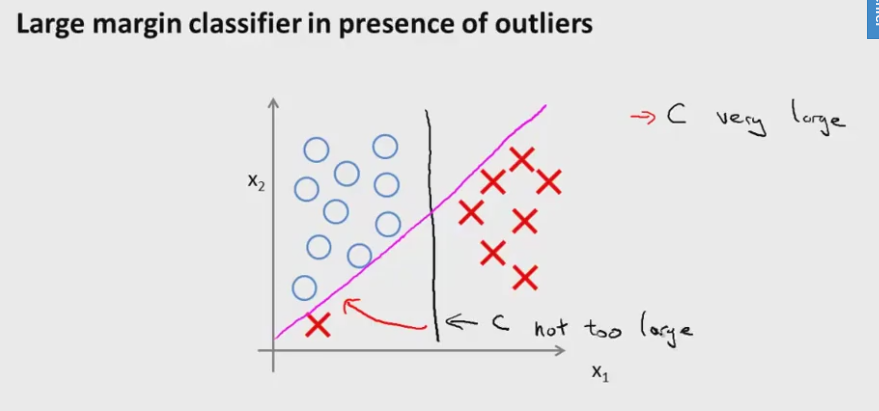
\includegraphics[scale=0.5]{sections/cs229/w9/outlier.png}
	\end{center}
\end{itemize}

\subsubsection{Mathematics Behind Large Margin Classification}
\begin{itemize}[--]
	\item In the case of 2 features, where $\theta_0=0$
		$$\min_{\theta}\frac{1}{2}\sum_{j=1}^{n}\theta_j^2=\frac{1}{2}||\theta||^2$$

		\begin{center}
			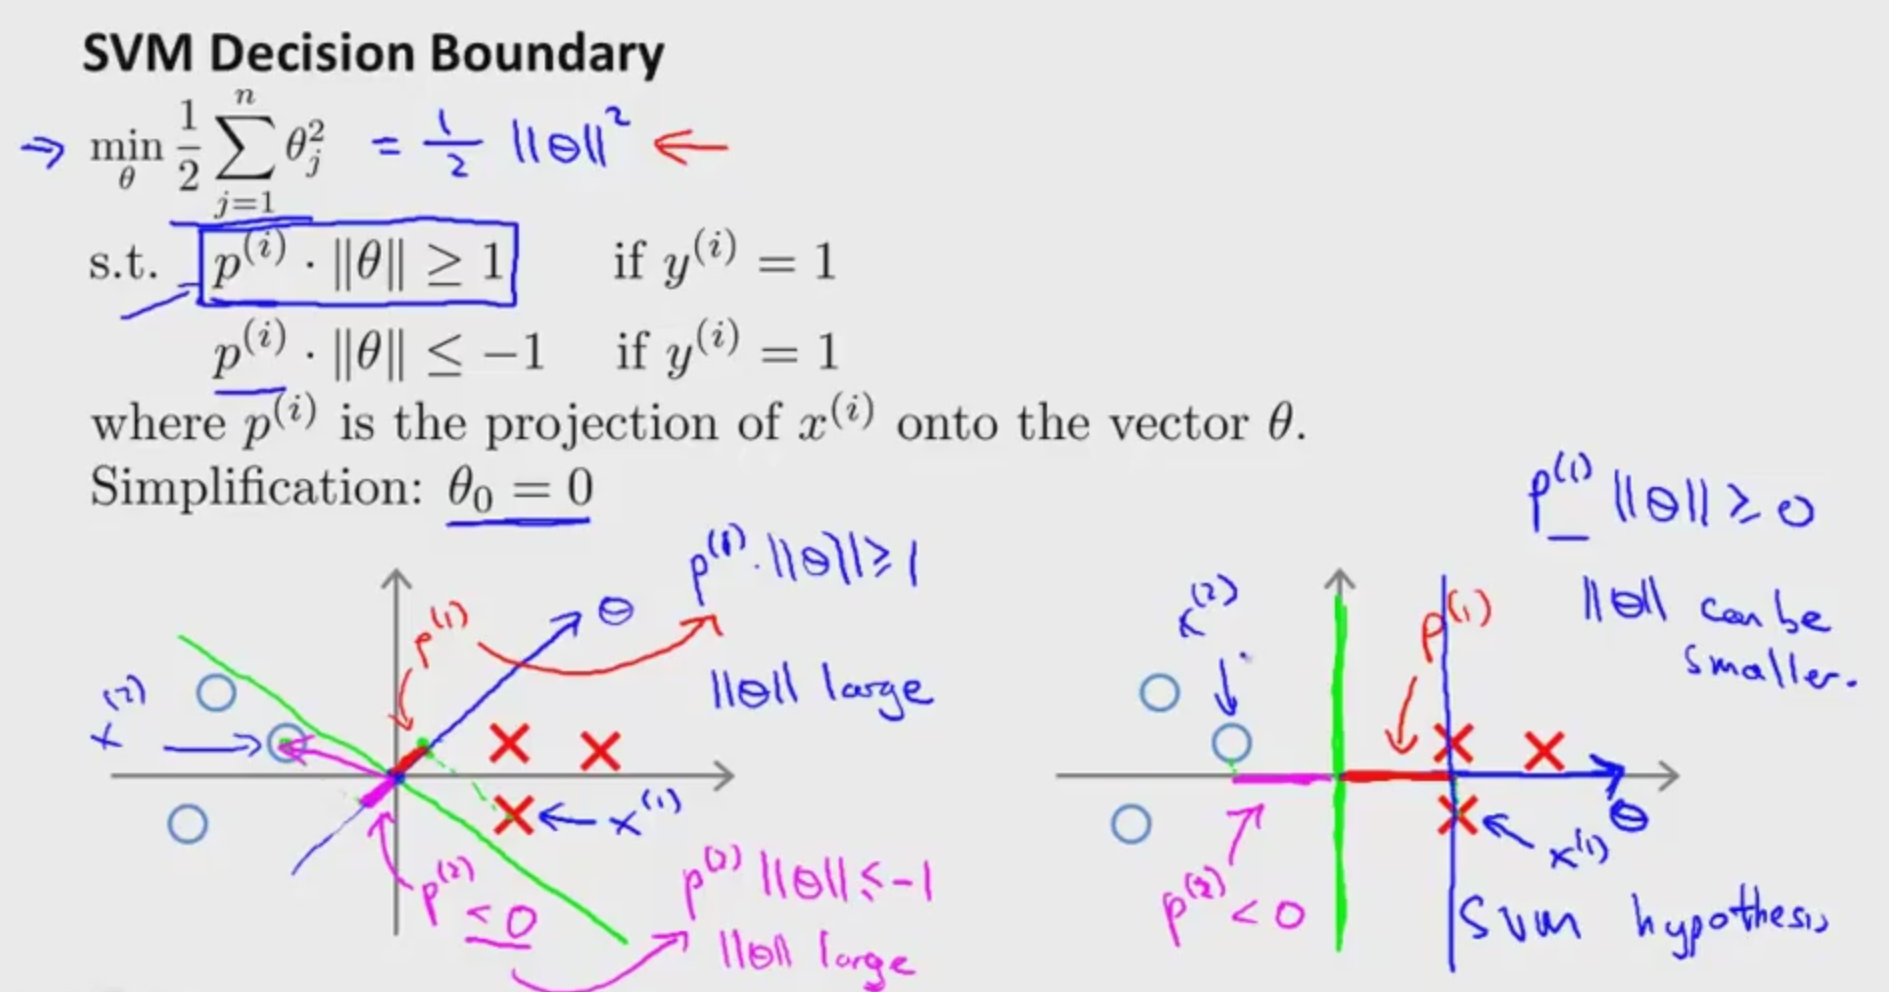
\includegraphics[scale=0.25]{sections/cs229/w9/boundary.png}
		\end{center}

	\item The margin works by trying to get the projectionss of the $y=1$ examples to be large positive values ($\theta$ points towards them, so they have large projections)
	\item This also results in very large negative values for the $y=0$
	\item The $\theta_0 = 0$ assumption, allows this simplification where decision boundary fits to the origin (the ideas proven here work $\theta\neq 0$ as well)
\end{itemize}

\subsubsection{Kernels I}
\begin{itemize}[--]
	\item One way to find a complex non-linear decision boundary is complex polynomials
	\item Another way to denote this is:
		$$\theta_0 + \theta_1 f_1 + \theta_2 f_2 + \ldots$$
	\item In this case:
		$$f_1=x_1, f_2=x_2, f_3=x_1 x_2, f_4=x_1^2, \ldots$$
	\item Is there a different/better chocie of the features $f_1, f_2,\ldots$?
	\item Given $x$, compute new feature depending on proximity to landmarks $l^{(1)}, l^{(2)}, l^{(2)}$
	\item One possible feature: $f_1=\text{similarity}(x,l^{(1)}=\text{exp}(-frac{||x-l^{(2)}||^2}{2\sigma^2})$
	\item For this example, we will also define our second \& third feature similarly: $f_n=\text{similarity}(x,l^{(n)})$
	\item This similarity function is called the \textbf{gaussian kernels}
	\item The idea of the similarity function is called the \textbf{kernel}
	\item If $x\approx l^{(1)}$, then $f_1=\approx \text{exp}(-\frac{0^2}{2\sigma})\approx 1$
	\item If $x$ is far from $l^{(1)}$ then $f_1\approx 0$
	\item So these measure how close $x$ is to the landmarks
	\item You can consider a guassian curve on the 3rd dimension, where the closer you get to the landmark, the higher up the hill (the corresponding value of the feature)
	\item As you increase $\sigma^2$ the value falls away much slower (higher variance tolerated)
	\item Example:
	\begin{center}
		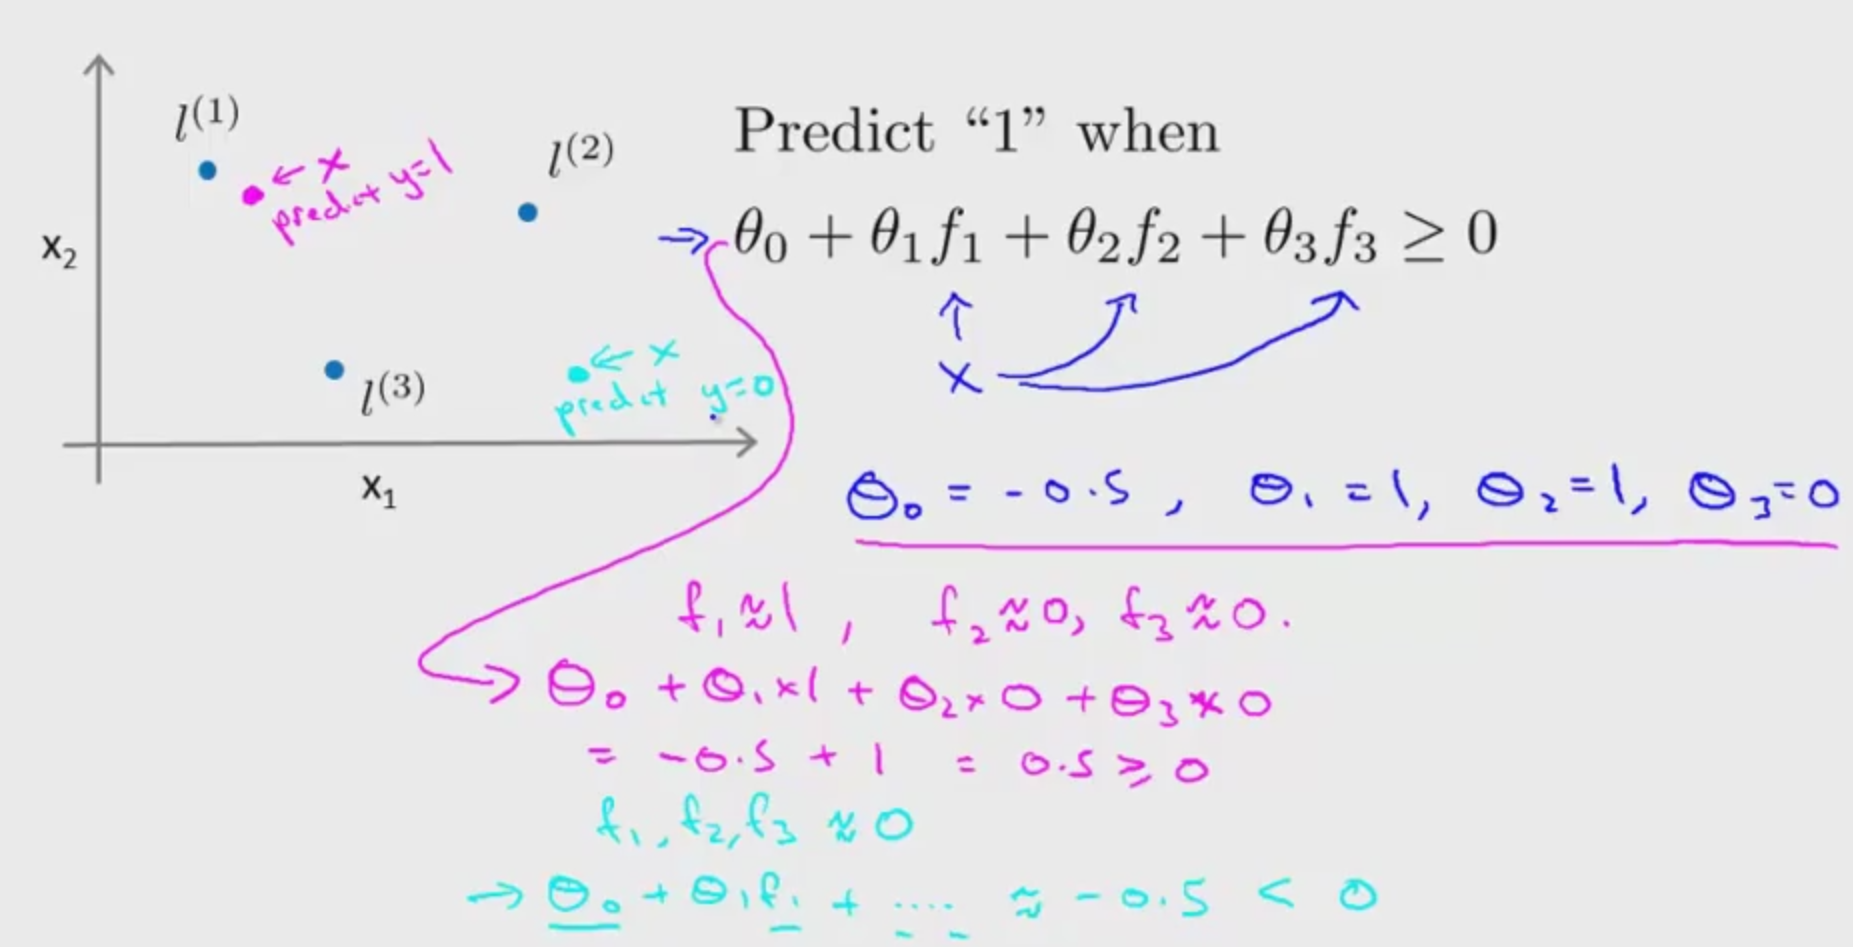
\includegraphics[scale=0.25]{sections/cs229/w9/ex_lm.png}
	\end{center}
\end{itemize}

\subsubsection{Kernels II}
\begin{itemize}[--]
	\item Where do we get $l^{(1)}, l^{(2)}, \ldots$?
	\item Given $m$ training examples, we choose $l^{(1)}, \ldots, l^{(m)}=x^{(m)}$
	\item And our features: $f_m=\text{similarity}(x, l^{(m)}$
	\item We can now represent our training example $i$ as a stacked vector all of all of the new features: 
		$$f^{(i)}=\begin{bmatrix}
			f_0^{(i)}\\
			\vdots \\
			f_m^{(i)}
		\end{bmatrix}$$

	\item SVM with Kernels
	\begin{itemize}[--]
		\item Hypothesis: Given $x$, compute features $f\in\mathbb{R}^{m+1}$
		\item Predict $y=1$ if $\theta^{T}f\geq 0$
		\item Training, by solving:
			$$\min_{\theta} C\sum_{i=1}^{m}y^{(i)}cost_i (\theta^{T}f^{(i)}) + (1-y{(i)})cost_0 (\theta^{T}f^{(i)}) + \frac{1}{2}\sum_{j=1}^{m}\theta_j^2$$
		\item Note: we are ignoring $\theta_0$ in our second term
	\end{itemize}

	\item SVM parameters:
	\begin{itemize}[--]
		\item One of the choices you need to make is what value of $C$ you would like to use
		\item Large $C$: lower bias, high variance
		\item Small $C$: higher bias, low variance
		\item We also need to choice $\sigma^2$
		\item Large $\sigma^2$: featurs $f_i$ vary more smoothly (varies slowly). Higher bias, lower variance.
		\item Small $\sigma^2$: features $f_i$ vary less smoothly (sharper change). Lower bias, higher variance
		\item 
	\end{itemize}
\end{itemize}

\subsubsection{Using an SVM}
\begin{itemize}[--]
	\item When using software packages to computer svm you need to specify:
	\begin{itemize}[--]
		\item Choice of parameter $C$
		\item Choice of kernel (similarity function)
		\item Choice of parameter $\sigma^2$
	\end{itemize}

	\item \textbf{Linear Kernel}: gives standard linear classifier
	\item Why might you choose a gaussian kernel? If $x\in\mathbb{R}^n$, n small andor large. Then the gaussian kernel can help with this very complex models
	\item If it asks you to provide a function to compute the kernel function, \textbf{perform feature scaling before using the kernel}
	\item Only kernels that satsify the condition ``Mercer's Theorem'' to make sure SVM packages' optimizations run correctly, and do not diverge
	\item Many off-the-shelf kernels available:
	\begin{itemize}[--]
		\item Polynomial kernel: $k(x,l;c,p)=(x^T l+c)^p,$
		\item More esoteric: string kernel, chi-square kernel, histogram intersection kernel, $\ldots$
	\end{itemize}

	\item Use the cross-validation set to decide on a kernel

	\item Many svm packages already ahve built-in multi-in multi-class classification unctionality. Otherwie, use one-vs-all method.

	\item Logistic regression vs. svm
	\begin{itemize}[--]
		\item If the number of training examples ($m$) is greater than the number of features ($n$), the typical approach is logistic regression over svm 
		\item If $n$ is small, and $m$ is intermediate ($n=1-1000,m=10-10000$) use svm with guassian kernel
		\item If $n$ is small and $m$ is large, create/add more features, then use logistic regression or svm without a kernel
		\item Neural network likely to work well for most of these settings, but may be slower to train
	\end{itemize}

	\item SVM is convex, so you will always find the global optimum
\end{itemize}